\documentclass[9pt, xcolor={usenames, dvipsnames}]{beamer}

\usepackage[sfdefault]{roboto}
\usepackage[utf8]{inputenc}
\usepackage[T1]{fontenc}
\usepackage{palatino}

\usepackage{styles/fluxmacros}
\usefolder{styles}
% Use Flux theme v0.1 beta
% Available style: asphalt, blue, red, green, gray 
\usetheme[style=flux]{flux}
\usetikzlibrary{hobby}

\usepackage{booktabs}
\usepackage{colortbl}
\usepackage{empheq}
\usepackage{xcolor}

\usepackage{caption}
\usepackage{subcaption}
\setbeamertemplate{caption}[numbered]
\captionsetup[figure]{font=footnotesize,labelfont=footnotesize}

\title{FDTD Underwater Acoustic Propagation}
\subtitle{Application to localization using interval analysis}
\author{Quentin Brateau}
\institute{ENSTA Bretagne~~~·~~~Agence Innovation Défense\\[0.5cm]
\includegraphics[width=0.5\textwidth]{images/logos_title_page.png}}
\date{\today}
\titlegraphic{images/logos_bw.png}

% \usepackage[usenames, dvipsnames]{xcolor}
\usepackage{pifont}
\newcommand{\cmark}{\textcolor{ForestGreen}{\ding{51}}}
\newcommand{\xmark}{\textcolor{Red}{\ding{55}}}

\usepackage{graphicx}
\usepackage{multimedia}
\usetikzlibrary{overlay-beamer-styles}

\usepackage[backend=biber,style=ieee]{biblatex}
\addbibresource{bib/presentation.bib}

\begin{document}

	\titlepage

	\part{Introduction}

		\begin{frame}{Introduction}{Financing of the works}
			\centering
			\begin{minipage}[c]{0.55\textwidth}
				\begin{block}{Research laboratory}
					\begin{itemize}
						\item ENSTA Bretagne
					\end{itemize}
				\end{block}

				\begin{block}{Projects}
					\begin{itemize}
						\item \textbf{DGA RAPID PROTEUS} :\\ Underwater acoustic propagation simulation using Finite Difference Time Domain (FDTD)
						\item \textbf{DGA ROBOTIX} :\\ Underwater acoustic source localization using interval analysis
					\end{itemize}
				\end{block}
			\end{minipage}
			\hfill
			\begin{minipage}[c]{0.4\textwidth}
				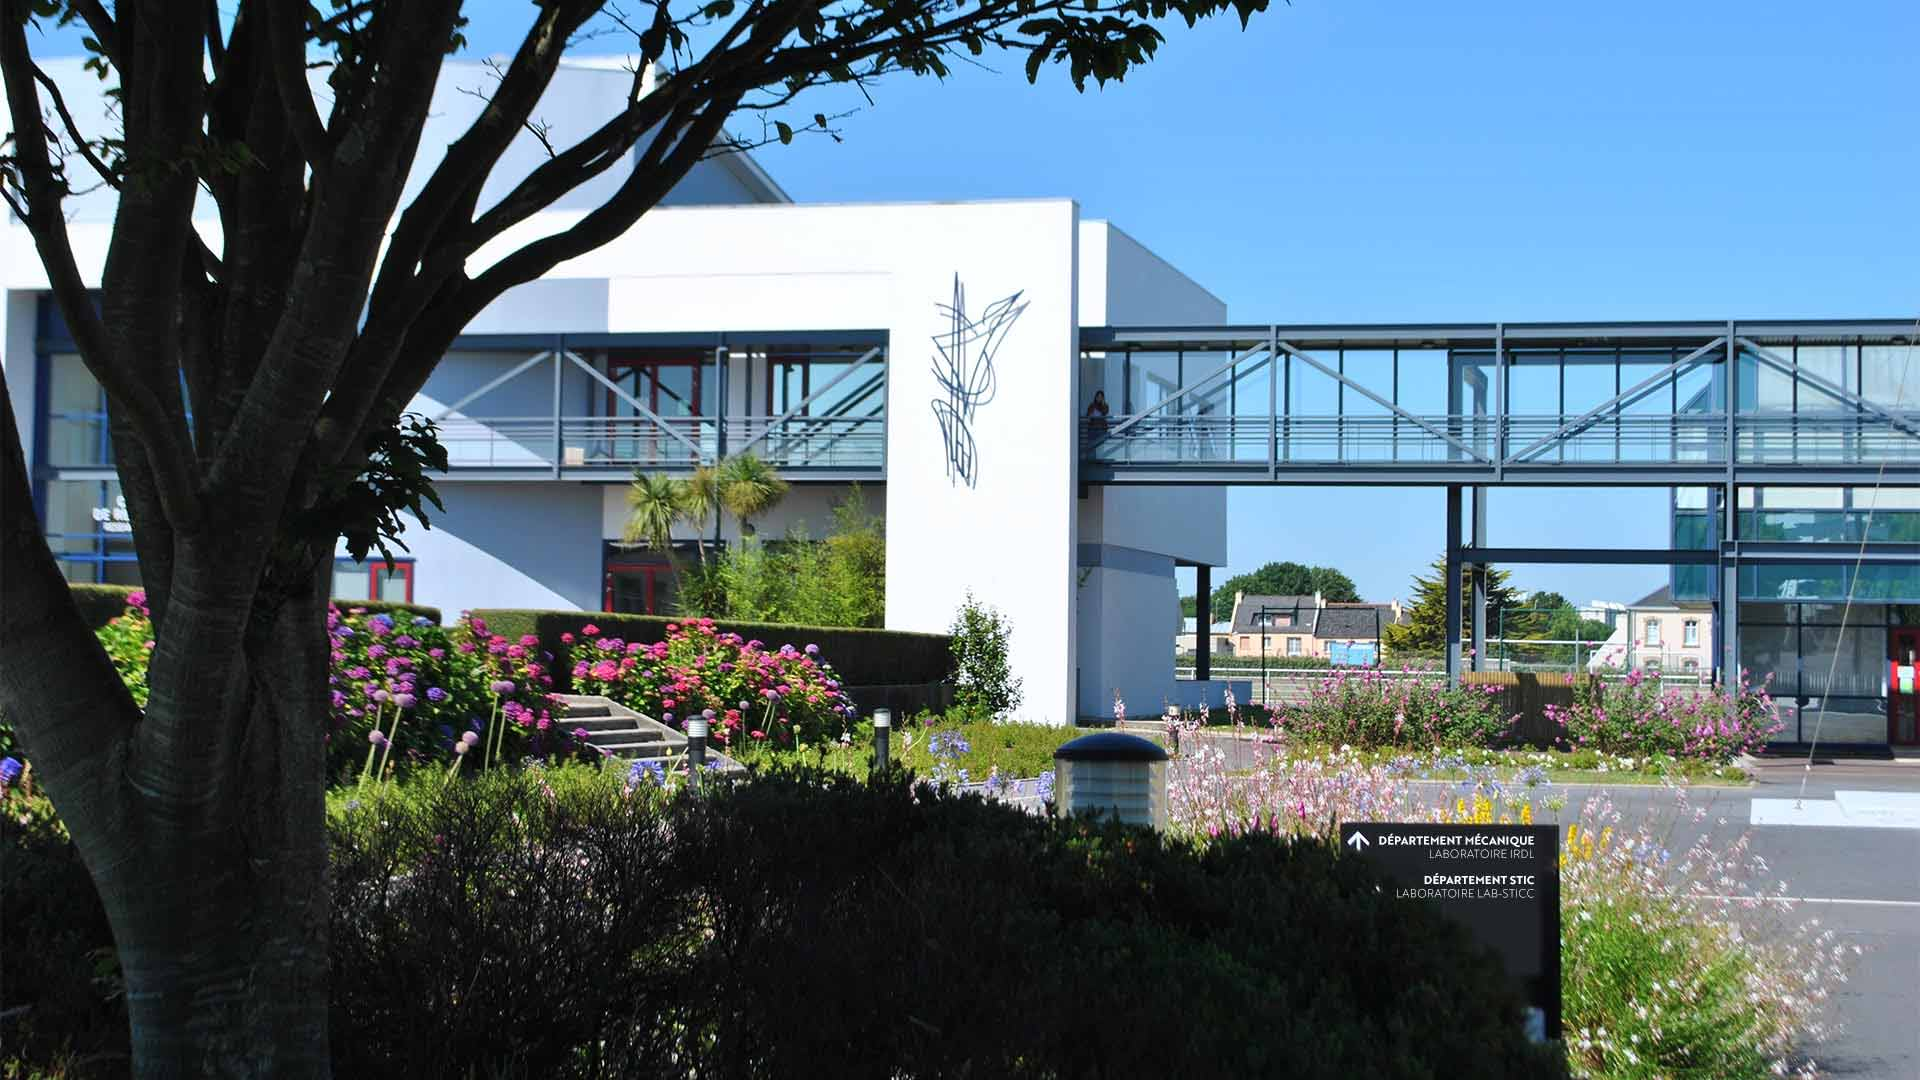
\includegraphics[height=0.7\textheight, trim={24cm 0 16cm 0}, clip]{images/ensta.jpg}
			\end{minipage}
		\end{frame}

	\part{Underwater acoustic propagation simulation using Finite Difference Time Domain}

		\begin{frame}
			\frametitle{Table of contents}
			\tableofcontents%[hideallsubsections]
		\end{frame}

		\section{Introduction}
		% \AllSectionsWithTitlePage

			\subsection{Scope of the study}

				\begin{frame}{Introduction}{Scope of the study}
					\centering
					\begin{minipage}{0.6\textwidth}
						\begin{block}{Variables of interest}
							\begin{itemize}
								\item Pressure
								\item Particle velocity
							\end{itemize}
						\end{block}
						\begin{block}{Scope of the simulation}
							\begin{itemize}
								\item Rectilinear Grid support for fields
								\item Linear acoustic approximation
								\item Viscoelastic modeling of materials
							\end{itemize}
						\end{block}
					\end{minipage}
				\end{frame}

			\subsection{Wave equation}

				\begin{frame}{Introduction}{Wave Equation}
					\centering
					\begin{minipage}[c]{0.3\textwidth}
						\begin{figure}
							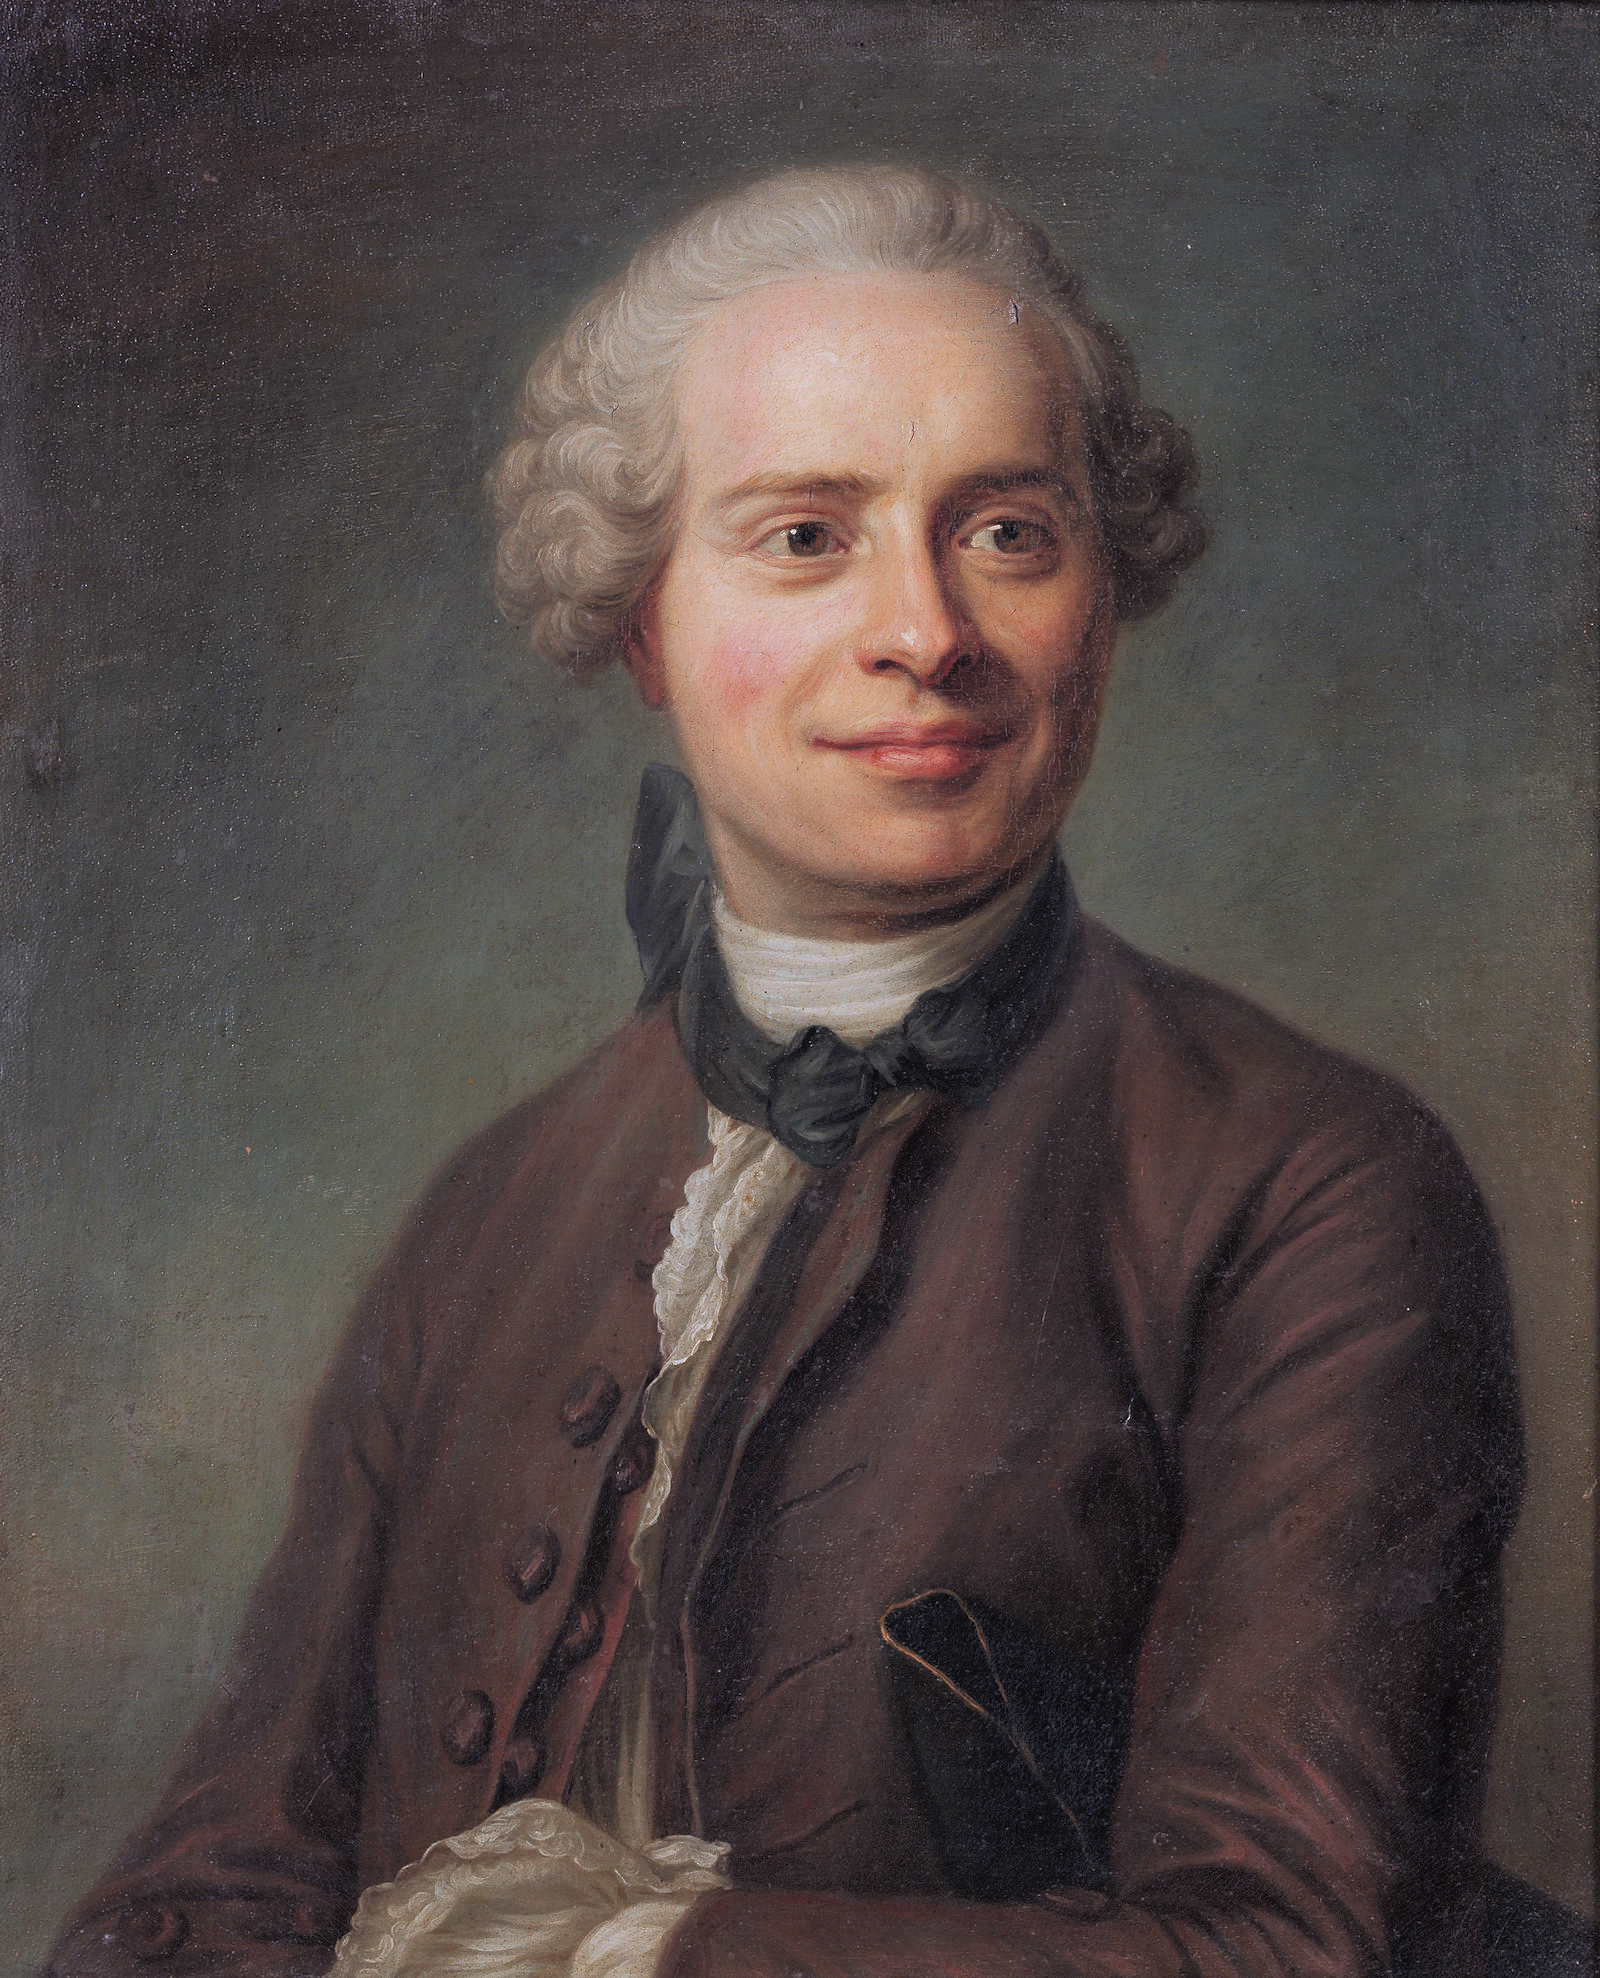
\includegraphics[width=\textwidth]{images/profile/Jean_Le_Rond_d'Alembert,_by_French_school.jpg}
							\caption{Jean Le Rond d'Alembert}
						\end{figure}
					\end{minipage}
					\hfill
					\begin{minipage}[c]{0.6\textwidth}
						\begin{alertblock}{Wave equation}
							\begin{eqnarray}
								\left(\nabla^2 - \frac{1}{c^2} \frac{\partial^2}{\partial t^2} \right) \phi(\mathbf{r}, t) & = & f(\mathbf{r}, t) \label{equation:alembert}
							\end{eqnarray}
							\begin{itemize}
								\item $\mathbf{r}$ : position
								\item $t$ : time
								\item $\phi$ : field
								\item $c$ : celerity 
							\end{itemize}
						\end{alertblock}
					\end{minipage}
				\end{frame}

		\section{Finite Difference Time Domain (FDTD)}

			\subsection{Numeric Scheme}

				\begin{frame}{FDTD}{Formalism~\footfullcite{blanch1994FDTD}}
					\centering
					\begin{minipage}[c]{0.45\textwidth}
						\begin{block}{Variables of interest}
							\begin{itemize}
								\item Pressure $p(t, x)$ \\
								\item Particle Velocity $u(t, x)$
							\end{itemize}
						\end{block}
						\begin{block}{Numeric scheme}
							\begin{itemize}
								\item $2^{nd}$ order in time $\mathcal{O}(\Delta t^2)$\\
								\item $4^{th}$ order in space $\mathcal{O}(\Delta x^4)$
							\end{itemize}
						\end{block}
					\end{minipage}
					\hfill
					\begin{minipage}[c]{0.45\textwidth}
						\begin{figure}[!htb]
							\centering
							\resizebox{0.8\textwidth}{!}{
								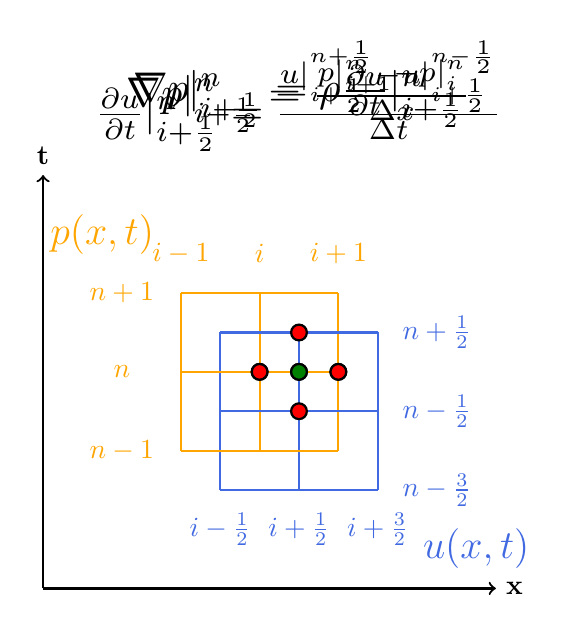
\begin{tikzpicture}
									\foreach \i in {-1,...,1} {
										\draw [Orange, thick] (\i,-1) -- (\i,1);
										\draw [RoyalBlue, thick] (\i+0.5,-1.5) -- (\i+0.5,0.5);
									}
									\foreach \i in {-1,...,1} {
										\draw [Orange, thick] (-1,\i) -- (1,\i);
										\draw [RoyalBlue, thick] (-0.5,\i-0.5) -- (1.5,\i-0.5);
									}
									\node[Orange] at (-2, 1.75) {\Large{$p(x, t)$}};
									\node[RoyalBlue] at (2.75, -2.25) {\Large{$u(x, t)$}};
					
									\node[Orange] at (-1.75, 1) {\normalsize{$n+1$}};
									\node[Orange] at (-1.75, 0) {\normalsize{$n$}};
									\node[Orange] at (-1.75, -1) {\normalsize{$n-1$}};
									\node[Orange] at (1, 1.5) {\normalsize{$i+1$}};
									\node[Orange] at (0, 1.5) {\normalsize{$i$}};
									\node[Orange] at (-1,1.5) {\normalsize{$i-1$}};
					
									\node[RoyalBlue] at (2.25, 0.5) {\normalsize{$n+\frac{1}{2}$}};
									\node[RoyalBlue] at (2.25, -0.5) {\normalsize{$n-\frac{1}{2}$}};
									\node[RoyalBlue] at (2.25, -1.5) {\normalsize{$n-\frac{3}{2}$}};
									\node[RoyalBlue] at (1.5, -2) {\normalsize{$i+\frac{3}{2}$}};
									\node[RoyalBlue] at (0.5, -2) {\normalsize{$i+\frac{1}{2}$}};
									\node[RoyalBlue] at (-0.5, -2) {\normalsize{$i-\frac{1}{2}$}};

									\draw[-to, >=latex, thick] (-2.75,-2.75) -- (3, -2.75) node[right] {$\mathbf{x}$};
									\draw[-to, >=latex, thick] (-2.75,-2.75) -- (-2.75, 2.5) node[above] {$\mathbf{t}$};

									\node[scale=1.5, visible on=<2-2>] at (0.5, 3.5) {$\nabla p|_{i+\frac{1}{2}}^n = \frac{p|_{i+1}^n - p|_i^n}{\Delta x}$};
									\draw[thick, black, fill=Red, visible on=<2-2>] (0,0) circle (0.1);
									\draw[thick, black, fill=Red, visible on=<2-2>] (1,0) circle (0.1);
									\draw[thick, black, fill=Green, visible on=<2-2>] (0.5,0) circle (0.1);
									
									\node[scale=1.5, visible on=<3-3>] at (0.5, 3.5) {$\frac{\partial u}{\partial t}|_{i+\frac{1}{2}}^n = \frac{u|_{i+\frac{1}{2}}^{n+\frac{1}{2}} - u|_{i+\frac{1}{2}}^{n-\frac{1}{2}}}{\Delta t}$};
									\draw[thick, black, fill=Red, visible on=<3-4>] (0.5,-0.5) circle (0.1);
									\draw[thick, black, fill=Red, visible on=<3-4>] (0.5,0.5) circle (0.1);
									\draw[thick, black, fill=Green, visible on=<3-4>] (0.5,0) circle (0.1);
									
									\node[scale=1.5, visible on=<4-4>] at (0.5, 3.5) {$\nabla p|_{i+\frac{1}{2}}^n = \rho \frac{\partial u}{\partial t}|_{i+\frac{1}{2}}^n$};
									\draw[thick, black, fill=Red, visible on=<4>] (0,0) circle (0.1);
									\draw[thick, black, fill=Red, visible on=<4>] (1,0) circle (0.1);
							\end{tikzpicture}}
							\caption{Staggered pressure and particle velocity fields}
							\label{fig:staggered}
						\end{figure}
					\end{minipage}
				\end{frame}

			\subsection{Viscoelastic modeling of materials}

				\begin{frame}{FDTD}{Viscoelastic modeling of materials}
					\centering
					\begin{minipage}[c]{0.3\textwidth}
						\begin{figure}
							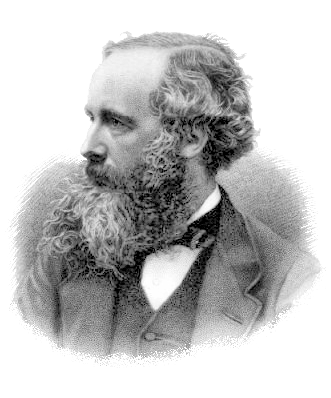
\includegraphics[width=\textwidth]{images/profile/James_Clerk_Maxwell.png}
							\caption{James Clerk Maxwell}
						\end{figure}
					\end{minipage}
					\hfill
					\begin{minipage}[c]{0.6\textwidth}
						\begin{block}{Standard Linear Solid (SLS) model}
							\begin{itemize}
								\item Viscoelastic material modeling 
								\item Springs
								\item Dashpots
							\end{itemize}
						\end{block}
						\begin{figure}
							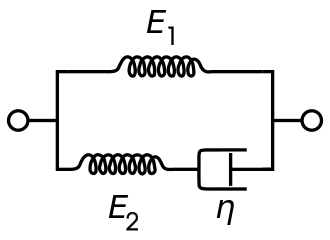
\includegraphics[width=0.4\textwidth]{images/SLS.png}
							\caption{Standard Linear Solid model, Maxwell representation}
						\end{figure}
					\end{minipage}
				\end{frame}

				\begin{frame}{FDTD}{Viscoelastic modeling of materials~\footfullcite{blanch1995Q}}
					\begin{minipage}[t]{0.48\textwidth}

						\begin{alertblock}{Constant Q modeling}
							\begin{equation}
								Q^{-1}(\omega) \approx \sum_{l=1}^L \frac{\omega \tau_{\sigma l} \tau}{1 + \omega^2\tau_{\sigma l}^2}
							\end{equation}
							\begin{itemize}
								\item $Q$ : Desired quality factor 
								\item $\omega$ Pulsation
								\item $L$ : Number of SLS
								\item $\tau_{\sigma l}$ : Relaxation constraint
								\item $\tau$ : Computed constant for material
							\end{itemize}
						\end{alertblock}
					\end{minipage}
					\hfill
					\begin{minipage}[t]{0.48\textwidth}
						\begin{figure}
							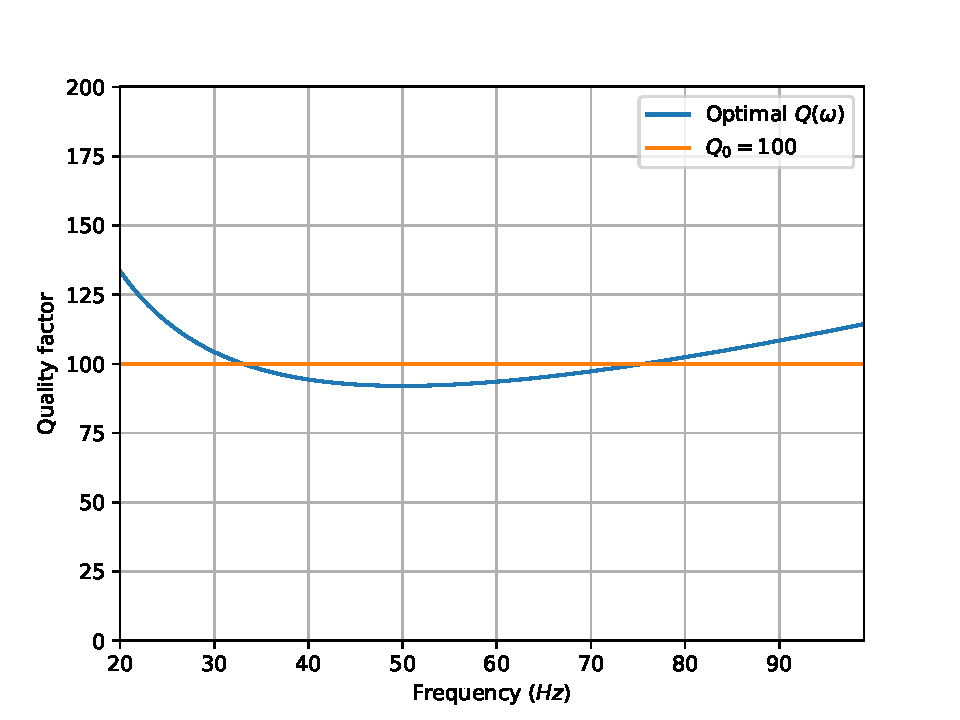
\includegraphics[width=\textwidth]{images/quality_factor.pdf}
							\caption{Optimal quality factor over a frequency range}
						\end{figure}
					\end{minipage}
				\end{frame}

		\section{Results}

			\subsection{Example}

				\begin{frame}{Results}{Example}
					\centering
					\begin{minipage}[c]{0.45\textwidth}
						\begin{figure}
							\movie{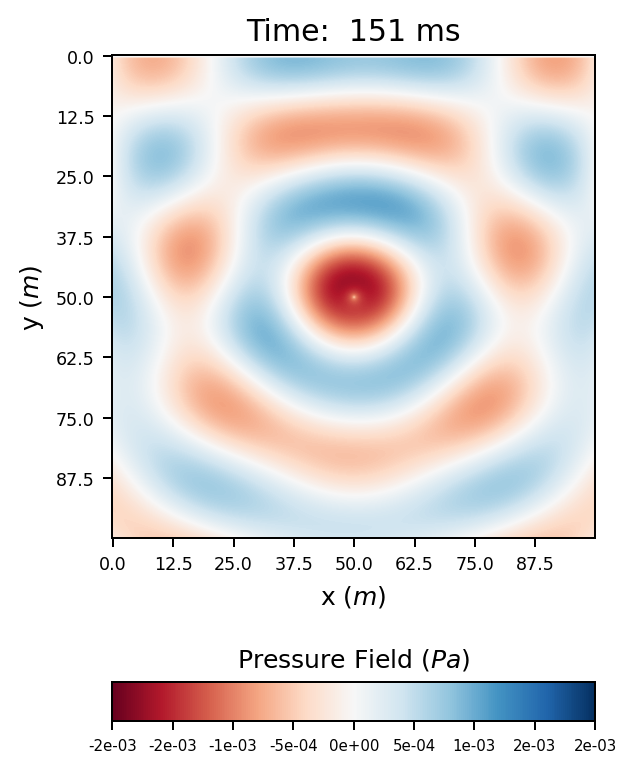
\includegraphics[width=\textwidth]{images/sphere/2dfdtd_00150.png}}{sphere.mp4}
						\end{figure}
					\end{minipage}
					\hfill
					\begin{minipage}[c]{0.5\textwidth}
						\begin{exampleblock}{Pulsing sphere}
							\begin{itemize}
								\item $(100,\ 100)\ m$ scene
								\item Emitter at $(50,\ 50)\ m$
								\item Reflection at the top
							\end{itemize}
						\end{exampleblock}
					\end{minipage}
				\end{frame}

	\part{Underwater acoustic source localization using interval analysis}

		\begin{frame}
			\partpage
		\end{frame}

		\begin{frame}
			\frametitle{Table of contents}
			\tableofcontents%[hideallsubsections]
		\end{frame}

		\section{Modeling}

			\subsection{Scene}

				\begin{frame}{Modeling}{Scene}
					\begin{figure}[!htb]
						\centering
						\resizebox{0.8\textwidth}{!}{
						\begin{tikzpicture}
							\coordinate (A) at (0,0);
							\coordinate (B) at (0,4);
							\coordinate (C) at (8,4);
							\coordinate (D) at (8,0);
			
							\fill[Apricot!80] (A) -- ($(A)!0.3!(B)$) -- ($(D)!0.3!(C)$) -- (D) -- cycle;
							\fill[ProcessBlue!40] ($(A)!0.3!(B)$) -- (B) -- (C) -- ($(D)!0.3!(C)$) -- cycle;
							\node at ($(A)!0.5!(D)+(0,0.55)$) {Sediments};
							\node at ($(A)!0.5!(D)+(0,2.25)$) {Water};
							\draw[fill=Red] ($(A)!0.75!(B)$)  arc (-90:90:0.18) -- cycle;
							\node at ($(A)!0.79!(B)+(1,0)$) {Emitter};
							\draw[fill=Green] ($(D)!0.64!(C)$)  arc (90:270:0.18) -- cycle;
							\node at ($(D)!0.6!(C)-(1,0)$) {Receiver};
							\draw (A) -- (B) -- (C) -- (D) -- cycle;
			
							\draw[to-to,>=latex] ($(A)-(0,0.3)$) -- node[below] {$r$} ($(D)-(0,0.3)$) ;
							\draw[to-to,>=latex] ($(A)-(0.7,0)$) -- node[left] {$z$} ($(B)-(0.7,0)$);
							\draw[to-to,>=latex] ($(A)!0.8!(B)-(0.1,0)$) -- node[left] {$z_e$} ($(B)-(0.1,0)$);
							\draw[to-to,>=latex] ($(D)!0.6!(C)+(0.1,0)$) -- node[right] {$z_r$} ($(C)+(0.1,0)$);
							\draw[to-to,>=latex] ($(A)-(0.1,0)$) -- node[left] {$h$} ($(A)!0.3!(B)-(0.1,0)$);
						\end{tikzpicture}}
						\caption{Modeling of the scene}
						\label{fig:scene}
					\end{figure}
				\end{frame}

	

		\section{Localisation Ensembliste}


		\subsection{Localisation ensembliste de source acoustiques}

			\begin{frame}{Acoustic reciprocity~\footfullcite{rayleigh1896theory}}
				\centering
				\begin{minipage}[c]{0.3\textwidth}
					\begin{figure}
						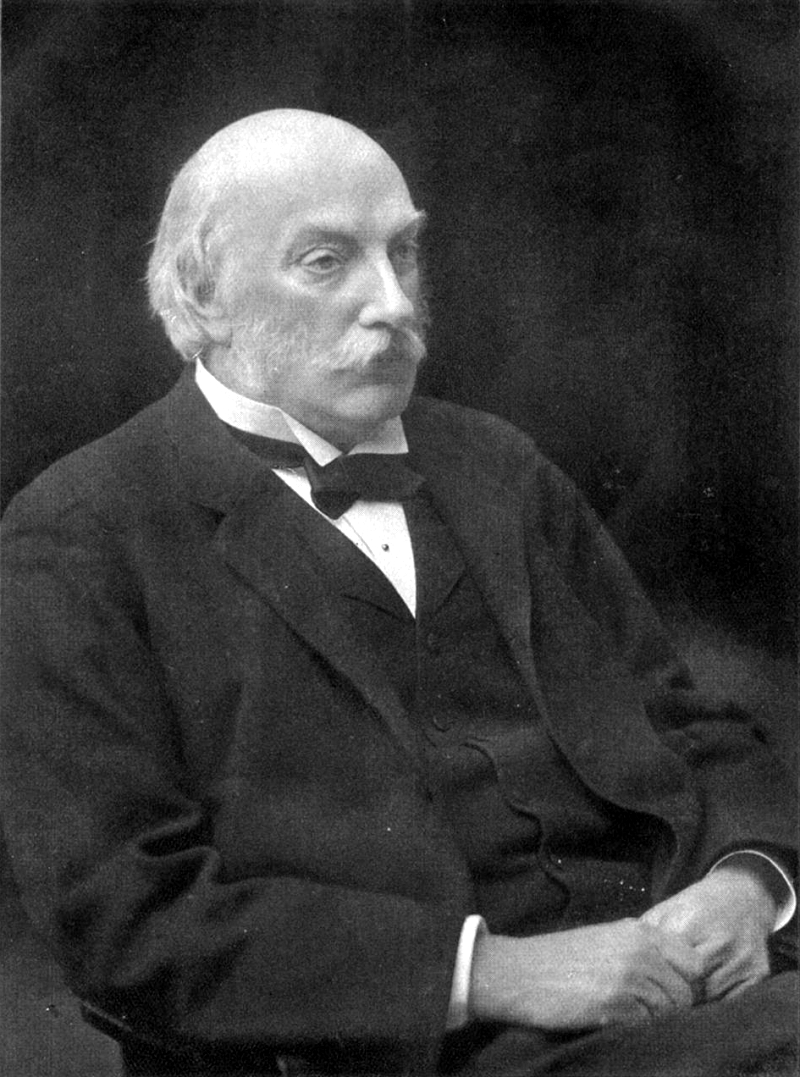
\includegraphics[width=\textwidth]{images/profile/John_William_Strutt.jpg}
						\caption{John William Strutt, $3^{rd}$ Baron of Rayleigh}
					\end{figure}
				\end{minipage}
				\hfill
				\begin{minipage}[c]{0.6\textwidth}
					\begin{block}{Acoustic reciprocity}
						\begin{itemize}
							\item Emitters $\leftrightarrow$ Receivers
							\item Efficient computation of the backward propagation
						\end{itemize}
					\end{block}
					\begin{block}{Assumptions}
						\begin{itemize}
							\item Field of linear acoustics
							\item Remains true in visoelastic environments
						\end{itemize}
					\end{block}
				\end{minipage}
			\end{frame}

			\begin{frame}{Problème d'inversion}
				\begin{figure}[!htb]
					\begin{subfigure}[!htb]{\textwidth}
						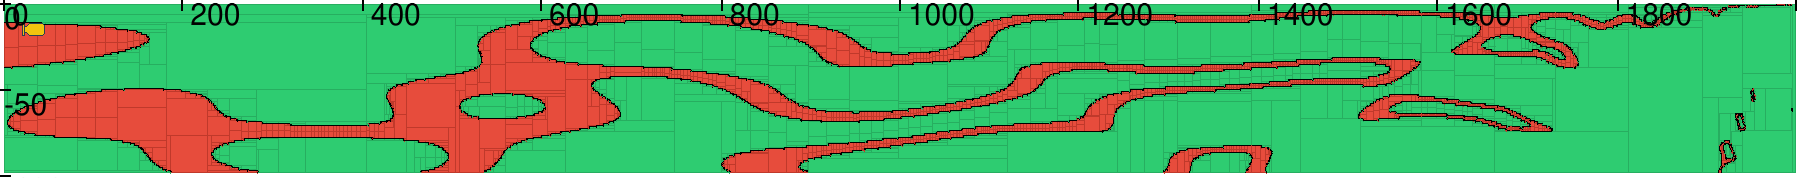
\includegraphics[width=\textwidth]{images/Hydrophone_20_2000.png}
						\caption{Compatibilité avec Hydrophone placé en $(2000, 20)\ m$}
					\end{subfigure}
					\begin{subfigure}[!htb]{\textwidth}
						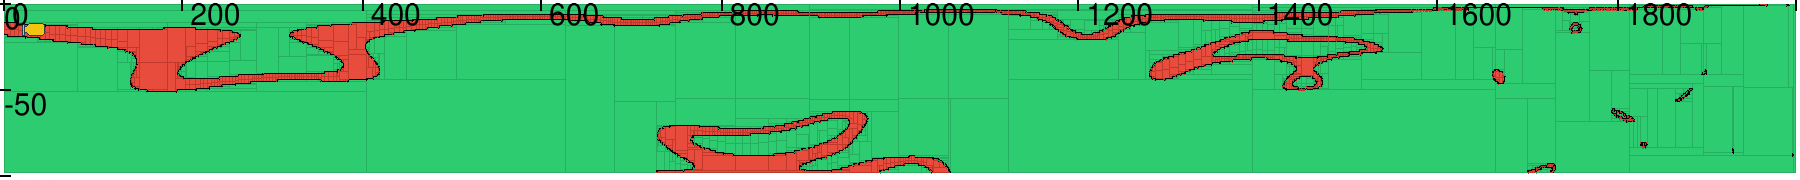
\includegraphics[width=\textwidth]{images/Hydrophone_40_2000.png}
						\caption{Compatibilité avec Hydrophone placé en $(2000, 40)\ m$}
					\end{subfigure}
					\begin{subfigure}[!htb]{\textwidth}
						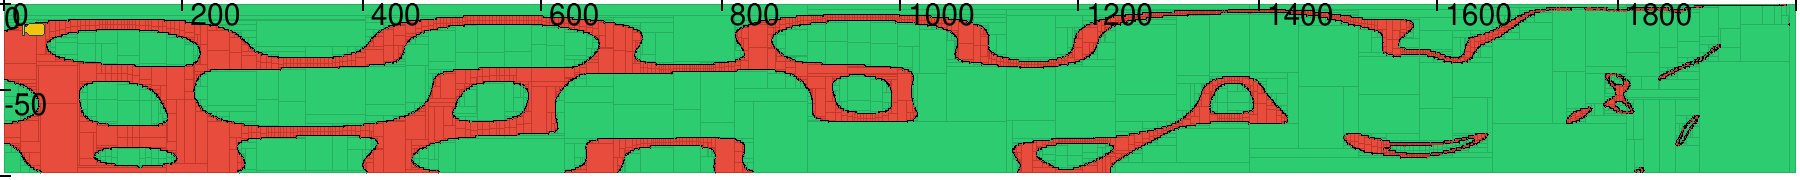
\includegraphics[width=\textwidth]{images/Hydrophone_60_2000.png}
						\caption{Compatibilité avec Hydrophone placé en $(2000, 60)\ m$}
					\end{subfigure}
					\begin{subfigure}[!htb]{\textwidth}
						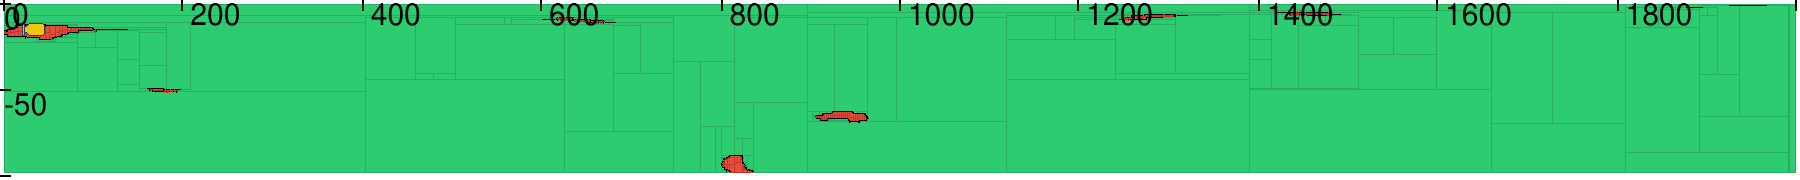
\includegraphics[width=\textwidth]{images/Proteus.png}
						\caption{Position de la source compatibles avec les mesures de niveaux acoustiques}
					\end{subfigure}
					\caption{Localisation ensembliste de la source acoustique}
				\end{figure}
			\end{frame}

		\section{Conclusion}
		
			\begin{frame}{Conclusion}
				\centering
				\begin{minipage}{0.55\textwidth}
					\begin{block}{Améliorations}
						\begin{itemize}
							\item Modélisation du bruit 
							\item Passage de la 2D à la 3D
							\item Passage du Python au C++
							\item Validation en milieu naturel
						\end{itemize}
					\end{block}

					\begin{block}{Localisation ensembliste}
						\begin{itemize}
							\item Émetteur/Récepteur en mouvement
							\item Simulation à plusieurs fréquences
							\item Navigation dans données sonar
							\item SLAM acoustique
						\end{itemize}
					\end{block}
				\end{minipage}
				\hfill
				\begin{minipage}{0.4\textwidth}
					\centering
					\begin{figure}
						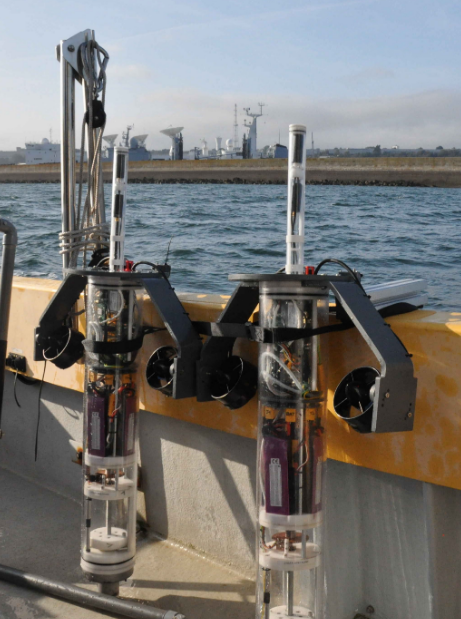
\includegraphics[width=0.8\textwidth]{images/seabot.png}
						\caption{SeaBot - Thomas Le Mézo}
					\end{figure}
				\end{minipage}
			\end{frame}
	
		\begin{frame}{Bibliographie}
			\printbibliography
			% \bibliography{bib/presentation.bib}
			% \bibliographystyle{ieeetr}
		\end{frame}
\end{document}